\chapter{OpenAUTOS}

Este capítulo apresenta a proposta do SO OpenAUTOS, destacando as escolhas tanto do projeto do software bem como a arquitetura de hardware adotada.

\section{Proposta}

O sistema OpenAUTOS é um SOE de código aberto, que busca atender a norma AUTOSAR SO, ou seja, realizar a implementação do sistema operacional proposto pelo padrão. Para tal, serão seguidas e respeitadas as guias e restrições definidas no relatório de especificações definidos em \citeonline{AUTOSAR:SOS}.

Por se tratar de um SO estático, não serão implementados gerenciadores de memória e sistemas de arquivos. Porém, isto implica que todas as tarefas, semáforos e demais objetos fornecidos pelo kernel sejam definidos em tempo de compilação. Segundo a norma, é obrigatório que um parser da linguagem OIL ou, alternativamente, \criarSigla[Linguagem de Marcação Extensível]{eXtensible Markup Language}{XML} seja fornecido, para que este faça a geração do arquivo de cabeçalho da linguagem C que será utilizado durante a compilação do SO. A \reffig{cap4_parser} ilustra este cenário.

\figura[]{cap4_parser}{Geração do cabeçalho de configuração}{7cm}{}

Na \reffig{cap4_arquitetura}, é apresentada uma lista dos módulos e objetos mais comuns em um SOE. O OpenAUTOS se propõe a implementar estes módulos, com exceção da alocação dinâmica de memória e sistema de arquivos pois, por se tratar de um SO estático, todas as alocações e definições deverão ser realizadas em tempo de compilação. Filas de mensagens e áreas de memória reservadas poderão ser definidas estaticamente.

\figura{cap4_arquitetura}{Módulos comuns a um SOE}{8cm}{}

Em termos de escalonador, o sistema deverá oferecer suporte para as tarefas normais e estendidas do padrão. As tarefas normais fazem uso de um escalonador de prioridades com Round Robin. Já as tarefas estendidas fazem uso de \emph{tabelas de escalonamento}, as quais garantem que restrições temporais serão atendidas e que uma operação não será interrompida antes de sua conclusão \cite{AUTOSAR:SOS}.

Segundo a norma \citeonline{AUTOSAR:SOS}, é necessário que a interface das funções sejam realizadas em C. Logo, está será a linguagem de implementação primária do projeto. Em seções críticas de performance, poderá ser utilizado a linguagem Assembly, mas nunca para a definição de métodos.

\section{Arquitetura}

Devido a disponibilidade, bem como o suporte as linguagens escolhidas, serão utilizadas as placas FRDM-KL25Z da \emph{freescale}, com processador \emph{ARM Cortex-M0}, ilustrado em \reffig{cap4_hardware_freescale}. Com base neste hardware, a implementação do OpenAUTOS utilizará uma arquitetura de processador único, centralizando todas as responsabilidades do SO em uma única ECU.

\figura{cap4_hardware_freescale}{FRDM-KL25Z}{7cm}{Freescale}

Para fins de simulações e demonstração, cada placa FRDM-KL25Z representará um sistema ou ECU de um veículo. Uma ECU será responsável por executar o SO OpenAUTOS, enquanto que as demais farão a manipulação de sistemas automotivos, como ABS, travamentos de portas, dentre outros, conforme ilustra a \reffig{cap4_arquitetura_comunicacao}

\figura{cap4_arquitetura_comunicacao}{Comunicação entre ECUs e Sistemas}{7cm}{}

Na comunicação entre os diferentes módulos eletrônicos serão utilizados os protocolos CAN e LIN. Será necessário o uso de dois pares de pinos TX/RX, um para cada protocolo. O protocolo LIN não precisa de nenhum tratamento especial, pois é baseado na UART. O procolo CAN, porém, não é disponibilizado nativamente. Sendo assim, serão utilizados \emph{transceivers} MPC2551 para comunicação entre ECUs.

A comunicação entre os diferentes módulos também deverá usar as normas do AUTOSAR para aplicativos, utilizando o interfaceamento definido na norma.

\section{Cronograma}

Com base no trabalho proposto, a Tabela \ref{tab:cap4_cronograma} propõe um cronograma para estudo e implementação do projeto.

\begin{table}[h!]
	\centering
	\caption{Cronograma.}
	\begin{tabular}{c}
		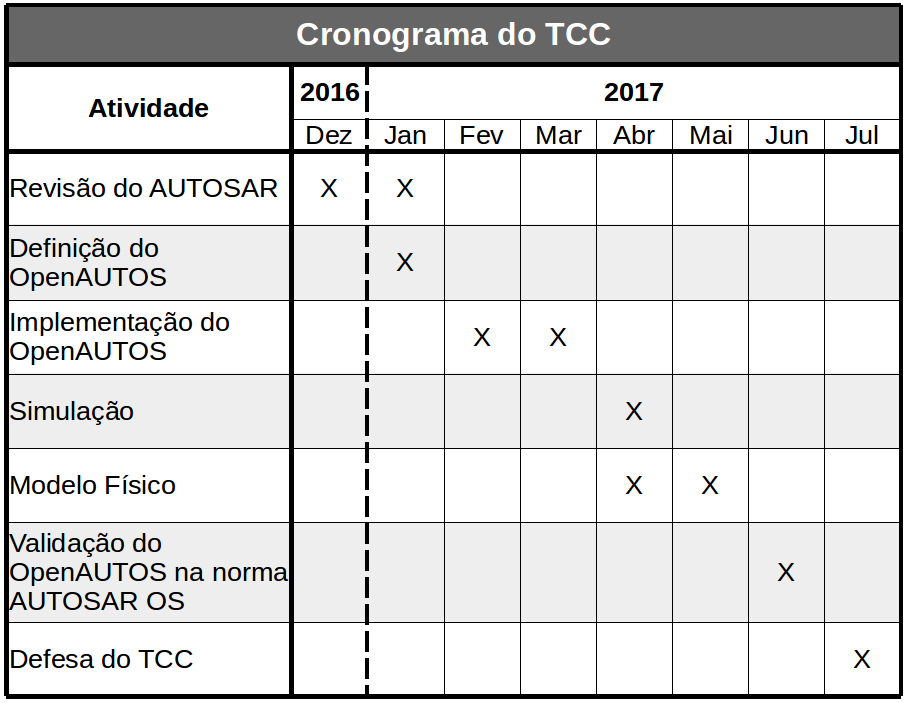
\includegraphics[width=\textwidth]{cap4_cronograma.png}		
	\end{tabular}
	\label{tab:cap4_cronograma}
\end{table}
